\chapter{Data Analysis}
\label{ch:lit_rev} 

The dataset used in this project is publicly available and can be accessed at \href{https://www.kaggle.com/datasets/zippyz/cats-and-dogs-breeds-classification-oxford-dataset}{Oxford Cats and Dogs Dataset}. It consists of 2 parts: images and annotations:

\section{Images} 
There are a total of 7384 images of pets, with 37 breeds
 present (both cats and dogs) which implies that there are 37 different classes in which the model can classify an image. These images are set in a variety of environments and locations, and are very different in style. Most importantly, they are casual pet pictures, which means that this solution can be used in real world applications where people with no experience and with no special equipment can use it.
 The following figure (Fig. 2.1) presents one image from breed present in the data set. These have been re shaped to be the same size of 299 x 299 pixels.\\   
\begin{figure}[h]
    \centering
    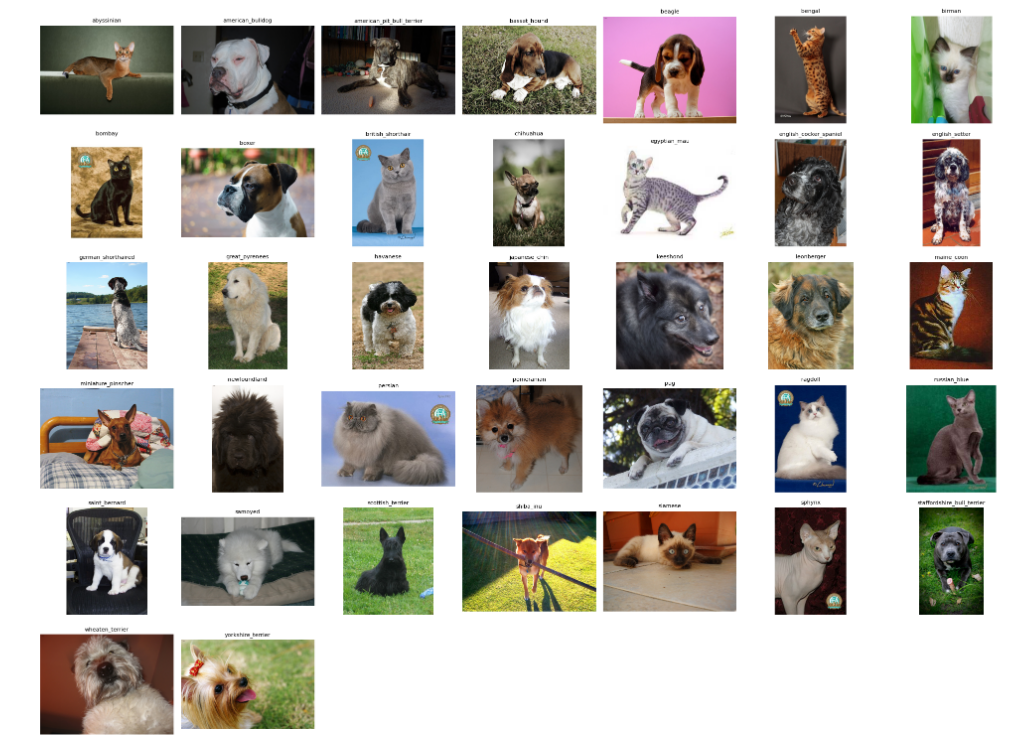
\includegraphics[width=0.7\textwidth]{figures/each_pic.png}
    \caption{One example image of each breed present in the dataset (resized to 299 x 299 pixels)}
    \label{fig:example_images}
\end{figure}
\noindent
It is important to guarantee that all classes have roughly the same representation in the data set to prevent the model from not learning all breeds equally. Thus it is important to understand the distribution of all classes. Breed-wise information can be seen in Fig. 2.2. For better understanding, I plotted the chart as seen in Fig 2.3.

\begin{figure}[h]
    \centering
    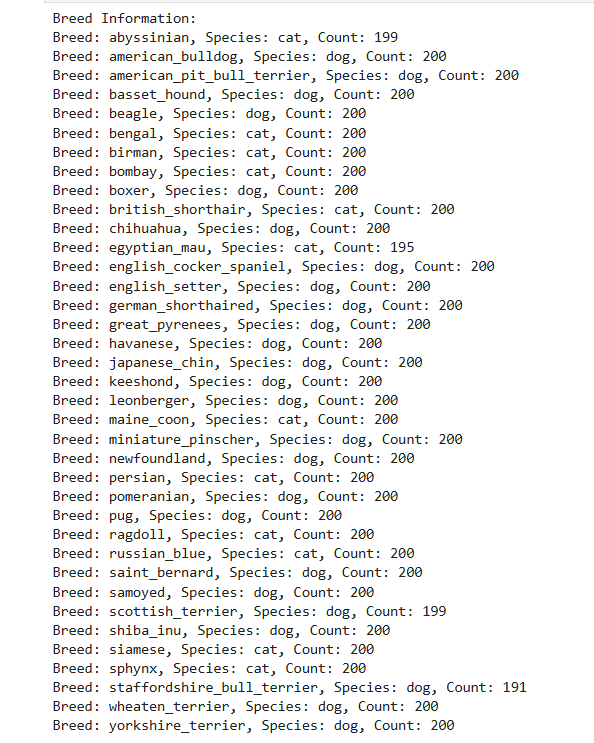
\includegraphics[width=0.7\textwidth]{figures/breeds.png}
    \caption{Images distribution over breeds}
    \label{fig:example_images}
\end{figure}
\begin{figure}[h]
    \centering
    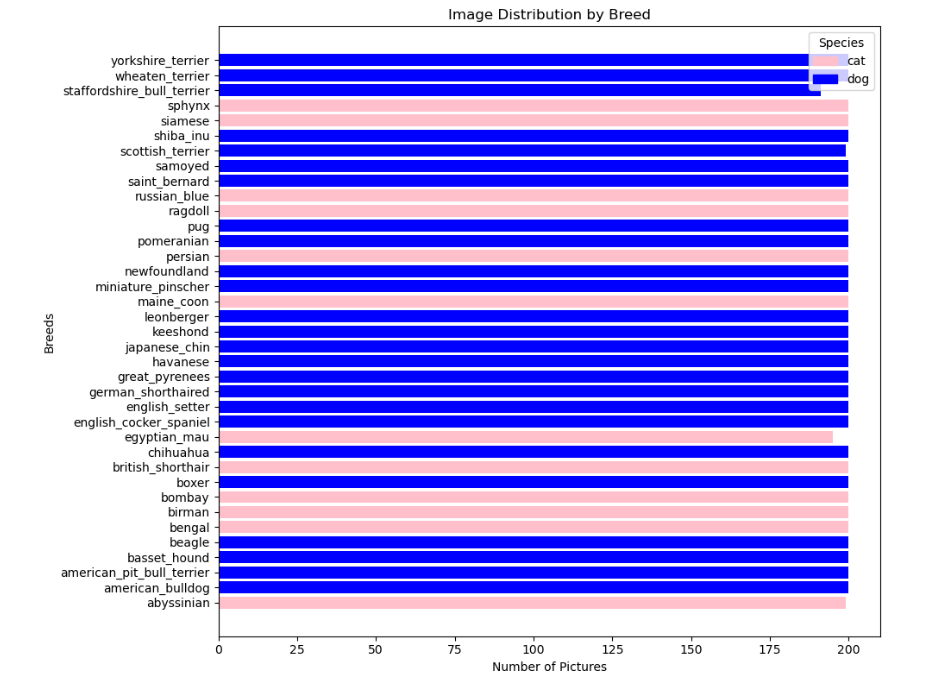
\includegraphics[width=0.7\textwidth]{figures/data.png}
    \caption{Graph representation of distribution}
    \label{fig:example_images}
\end{figure}
\clearpage
\noindent
It can be deduced that all breeds have similar representation in the data set. There is around 200 images of pets from each breed. It can also be seen that dogs have almost twice the number of images than cats. However, this won't affect the  model as the classifier isn’t trying to distinguish between those two classes, but between the 37 different breeds.
\section{Annotations}
The dataset also includes extra information, including:
\begin{itemize}
    \item \textbf{Trimap Annotations:} There is one trimap annotation for each picture indicating the pixels that are foreground and background. Background removal was done using this annotations.
    
    \item \textbf{Head Bounding Box Annotations:} Annotations in PASCAL VOC Format (not utilized in this project).
    
    \item \textbf{Other Documents:} Files such as a text file containing information for each image (class ID, species, etc), and two files describing possible train and test image splits.(not used in this project)
\end{itemize}

\section{Summary} 
This chapter outlined the Oxford Cats and Dogs Breeds Classification Dataset, consisting of 7,384 pet images across 37 breeds in diverse settings. Each breed is well-represented, making the dataset ideal for a robust classification model. The dataset also includes trimap annotations for background removal and other documents with metadata, laying the groundwork for accurate breed classification.
